\chapter{Data Collection Methodology}
\label{chapter:data}  

The goal of our work is to study real-world phenomena through social media.
%
Hence, we focus on the creation of a comprehensive event collection.
%
Our methodology consists in gathering tweets and then identifying coherent
real-world events. 
%
We use the Twitter Application Programming Interface~\cite{twitterapi}, or also
{\em Twitter API}, to retrieve tweets from Twitter. 
%
The data collection methodology resembles related work on identifying content
for planned events~\cite{Becker:2012}.
%
The main idea is to aim for high precision by retrieving news from trusted
sources, and then aiming for high recall by retrieving content from users about
the obtained news events from the trusted sources.
%
Our dataset consists of 20,066 news events. These events encompass 193,445,734
tweets, produced by 26,127,624 different users.

%%

Section~\ref{sec:dataset} describes the steps to follow to build the dataset,
while Section~\ref{sec:cleaning} describes data cleaning and validation.


\section{Building the Dataset}\label{sec:dataset}

The dataset was constructed using a set of seed Twitter accounts, from which
newsworthy messages were obtained.
%
From these messages, we identified relevant keywords which describe the current
event, and used them to retrieve tweets from the general public to improve
recall.
%
Finally, we grouped some of these sets into {\em events}.


% \begin{enumerate}
% \item \textbf{Tweet}: A social media object consisting of a text message with
%   metadata: author's data (name, followers, followees, etc.), date of
%   publication (timestamp), number of times it was \emph{retweeted} or re-shared,
%   etc.

% \item \textbf{Search Result}: A search result is a tuple consisting of a pair of
%   keywords and a date that represents it, and a set of tweets associated with
%   it, as every tweet message in the set contains both keywords.

% \item \textbf{Event}: An event is going to be considered as an extended version
%   of a search result. In other words, it is a tuple consisting of a set of
%   keywords, a date and a set of tweets. Each tweet message contains at least two
%   keywords of the keywords set. For example, Figure~\ref{fig:event-example}
%   shows an event consisting of three searches. An event is produced by joining
%   keywords from the search results, as described in Section~\ref{subsec:group}.
% \end{enumerate}

\subsection{Collecting related posts for news on Twitter}

The Twitter API~\cite{twitterapi} provides an interface to retrieve tweets in an
automated manner. For building a dataset of news events, it is necessary to
identify events from the Twitter stream.

Essentially, there are two ways to retrieve tweets from Twitter: using the
{\em Streaming API}, or the {\em REST API}. 
%
The Streaming API provides a way to retrieve real time tweets using zero or more
keywords to filter the stream. 
%
The amount of tweets that we can obtain is capped up to 1\% of the real stream
at a given moment\footnote{The \emph{Firehose} or full stream corresponds to the
full stream of tweets. The Streaming API samples up to 1\% of those tweets that
come every second. However, there was evidence that the Streaming API is not a
good random sample in some cases, for example, when looking for the top hashtags
in a period of time~\cite{morstatter2013sample}.}.  
%
The REST API allows us to get tweets from the past\footnote{However, the
documentation is not clear in terms of how long nor how many tweets can be
retrieved.}, by giving it a search term, consisting on one or more keywords. 
%
Both services return a set of tweets after a period of time. 

As our initial motivation was to study the characteristics of a news event as
soon as they break, we wanted to obtain as many tweets as possible from that
moment.
%
For that reason, it was necessary to obtain tweets about events event before
they were reported\footnote{Tweets related to the topic. For example, tweets
about Nelson Mandela before his death.}, and after that, to see the change in
volume.
%
With this in mind, we chose to use the REST API.

We manually crafted a set of about fifty verified news accounts in Twitter (such
as BBCNews, CNN, Al Jazeera, etc.). 
%
The full list of news sources can be found in Appendix~\ref{ape:news}.
%
Most of the news accounts are from the United States, or English spoken.
%
The list was made manually by performing a search for ``news'' in the Twitter
site\footnote{\url{https://twitter.com/search?q=news&src=typd&mode=users}} and
selecting verified users. 
%
Verified accounts are accounts that were verified for identity
authenticity\footnote{\url{https://support.twitter.com/articles/119135-faqs-about-verified-accounts}},
although how the process of verification is made is unknown outside Twitter. 

Each of these accounts posts messages about news, some of them breaking, and
sometimes they post advertising, etc. 
%
Let the tweets posted from those accounts be called \emph{headlines}. Some
examples of headlines are the following: 

{\it 
\begin{itemize}
\item @BBCNews: RT @BBCSport: FT: Uruguay 2-1 England. Two goals from
  Luis Suarez enough to beat \#ENG. <URL> \#WorldCup
  \#ENGvsURU <URL>…
\item @BreakingNews: Presbyterian General Assembly votes to allow
  pastors to preside at same-sex marriages - @AP
  <URL>
\item @Channel4News: Chile mountain top is blown off - in the name of
  astrophysics: <URL> \#c4news
\item @BBCNewsUS: Kevin McCarthy elected Republican House majority
  leader, party's second-ranking post <URL>
\end{itemize}
}

Our assumption is that if an important event is happening in a certain moment in
time, then several news accounts will be reporting on that event shortly after,
using similar vocabulary in their reporting.
%
From this assumption, we collected headlines every hour, identified the most
common keywords from the headlines, and used those keywords to search for more
tweets in the API.

\begin{figure}
\begin{center}
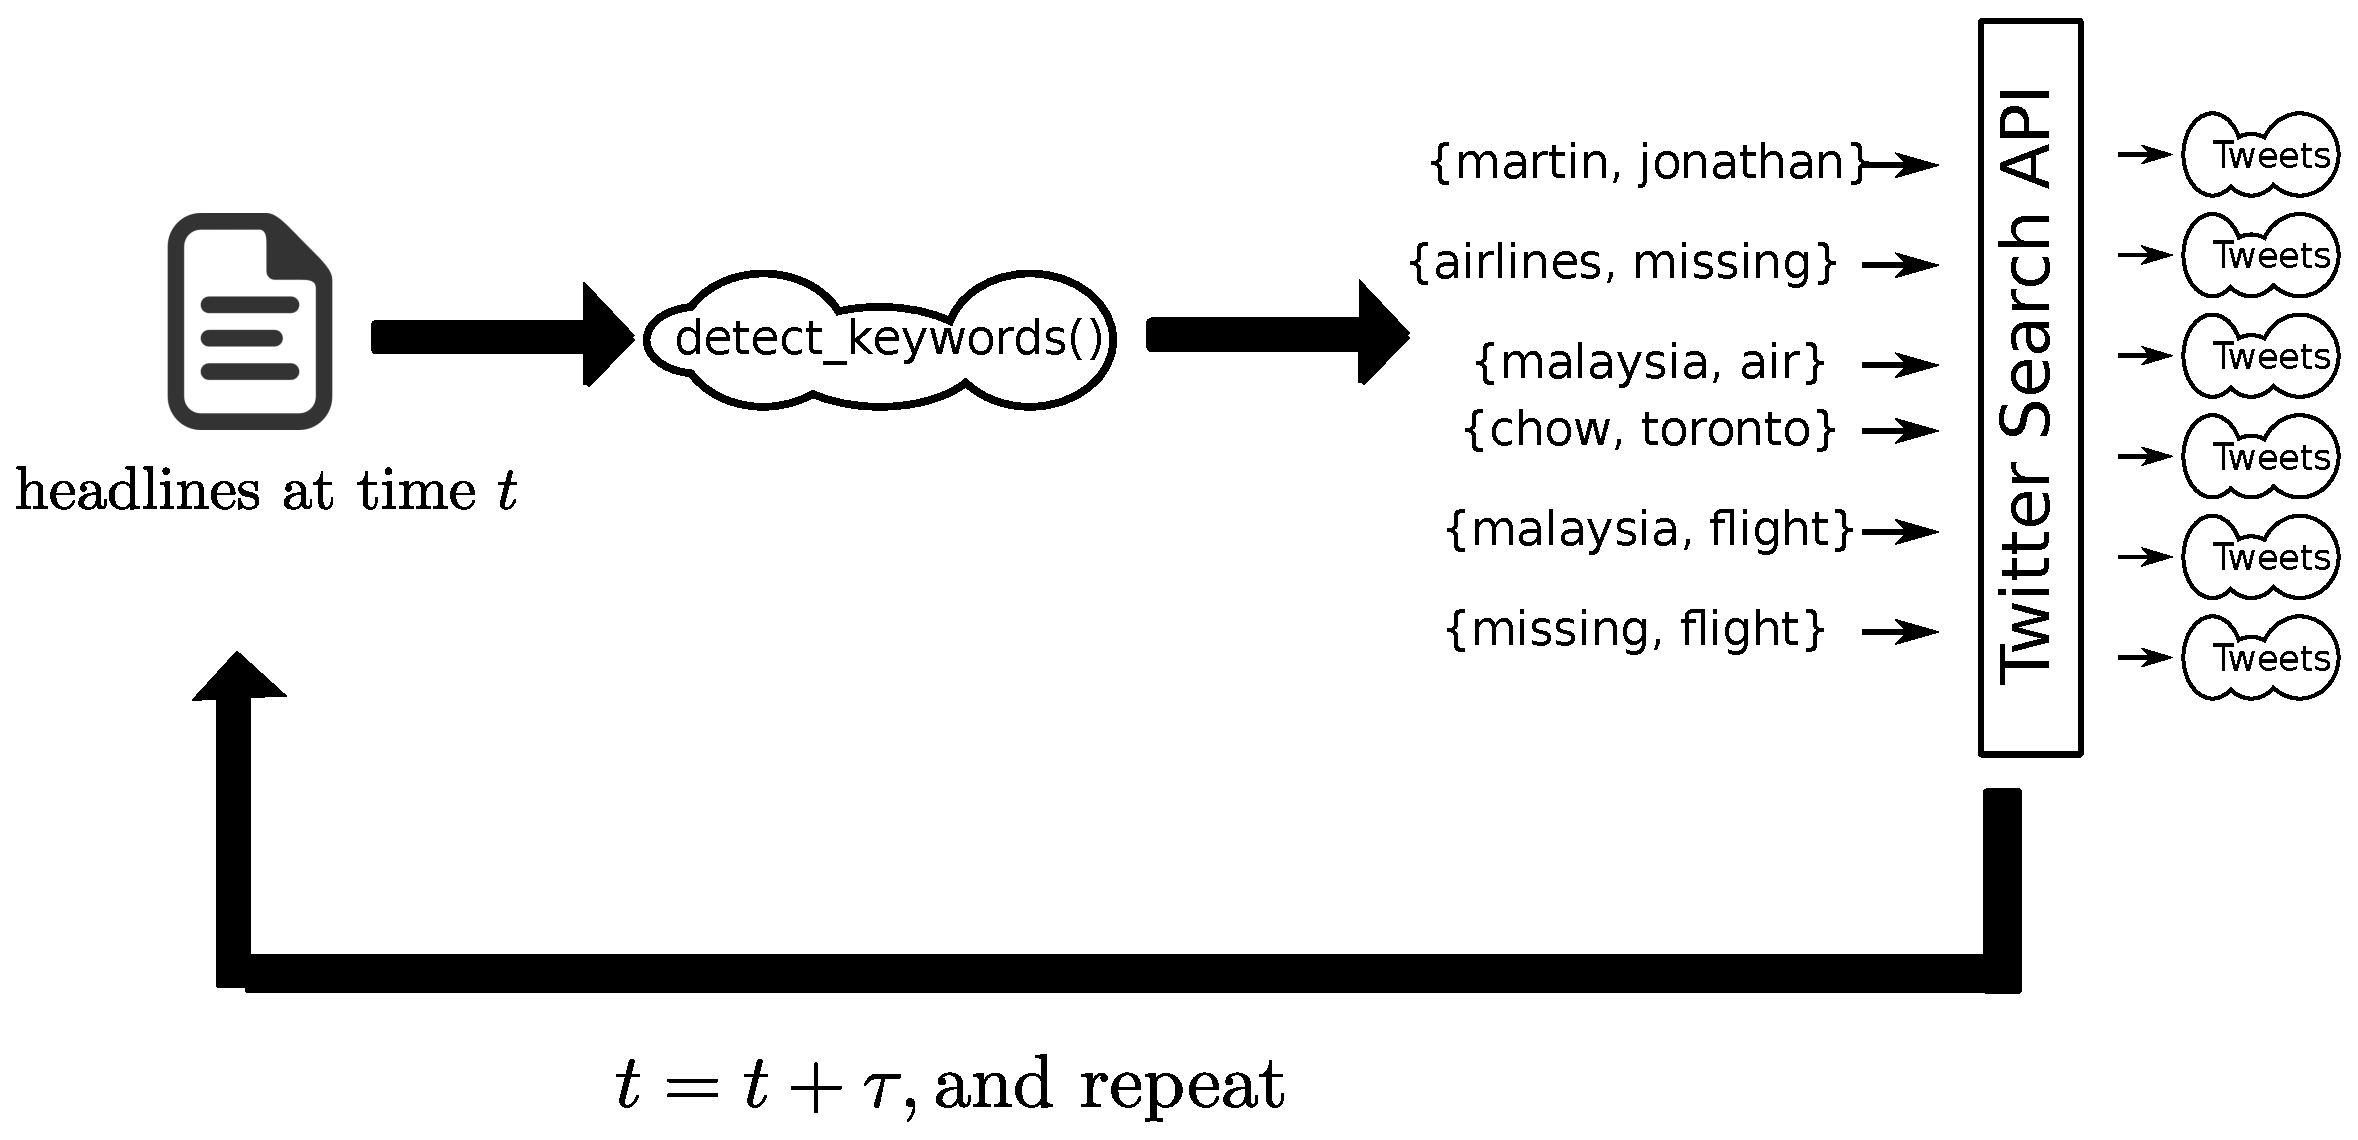
\includegraphics[width=\textwidth]{figures/data/data_collection_1}
\caption[Pipeline of data collection]{Pipeline of data collection. From the
  selected news accounts a set of headlines (tweets) are retrieved. Then, six
  pairs of keywords are identified based on the most frequent itemsets present
  in the headlines. Each pair of keywords is used as a search term of the
  Twitter REST API. For one hour, the process retrieves tweets related to each
  pair of keywords. After that, the process starts again for the next set of
  headlines.}
\label{fig:pipeline}
\end{center}
\end{figure}



Every $t=60$ minutes, all headlines posted in the last $t$ minutes are
retrieved using the API. 
%
We pre-process the retrieved headlines by removing stopwords, punctuation, URLs,
hashtags, mentions, and converting words to lowercase.
%
From the processed headlines the most frequent sets of words are then chosen.
%
From the resulting sets, the top $k=2$ words are chosen from each of the top
$g=6$ groups. 
%
Each pair of words, or keywords, are used as input for the REST API to retrieve
tweets related to the keywords. 
%
The main idea is that if several headlines discuss the same topic, then it is
considered an important topic, and users talk about it using some of the most
frequent words. 
%
We describe the algorithm to identify the frequent
itemsets~\cite{zaki2000scalable} in Algorithm~\ref{alg:detect_keywords}.
%


\renewcommand{\algorithmicrequire}{\textbf{Input:}}
\renewcommand{\algorithmicensure}{\textbf{Output:}}
\newcommand{\I}{\mathcal{I}}
\renewcommand{\G}{\mathcal{G}}
\newcommand{\ess}{\mathcal{S}}

\begin{algorithm}
\caption{Detect common keywords from headlines}
\label{alg:detect_keywords}
\begin{algorithmic}[1]
\REQUIRE A set of $M$ sets of words, $\ess= \{H_1,H_2, \ldots, H_M\}$, positive integers $k, \eta$
\ENSURE $k$ sets of keywords, $G = (\I_1,\I_2,\ldots,\I_{k})$
\STATE $\I_i \leftarrow \emptyset$ for $i = 1,2, \ldots,k$ %\COMMENT{Initialize item sets to empty sets}
\STATE $score_i \leftarrow$ empty dictionary for $i = 1, 2, \ldots,k$ %\COMMENT{Initialize keyword set scores to $1$}
\STATE $i \leftarrow 1$
\FOR{every pair of headlines $\{H_a, H_b\} \in \ess$ such that $|H_a \cap H_b| \geq \eta$}
    \STATE $\G \leftarrow H_a \cap H_b$ \label{alg:line:intersect} %\COMMENT{$\G$ is the set of common words of $H_a$ and $H_b$}
    \STATE $j \leftarrow \operatorname{arg\,max}_j |\I_j \cap \G|$
    \IF{$|\I_j \cap \G| \geq \eta$}
        \STATE $\I_j \leftarrow \I_j \cap \G$
        \STATE $score_{j}[w] \leftarrow score_{j}[w] + 1$ for all $w \in \I_j$
    \ELSE
        \STATE $\I_i \leftarrow \G$
        \STATE $score_{i}[w] \leftarrow 1$ for all $w \in \I_i$
        \STATE $i \leftarrow i + 1$
    \ENDIF
\ENDFOR
\STATE $total\_score_i \leftarrow \sum_{w \in \I_i} score_{i}[w]$ for $i=1,2,\ldots,k$
\RETURN $G = (\I_i$ sorted by $total\_score_i)$

\end{algorithmic}
\end{algorithm}

We only considered the top two keywords from each group, that is, we only
considered pairs of keywords from the headlines. 
%
This is because we use Twitter as our data source, and the tweets can be very
short (140 characters at most at the time of the data collection). 
%
Also, we selected only the top six groups, to obtain an acceptable rate of news
events per time unit. 
%
If there are not enough tweets or groups, we only choose the keywords available
for that period of time.

After one run of the process, a set of $g=6$ \emph{search results} or sets of
tweets are created and stored. 
%
A search is a tuple consisting of a pair of keywords and a set of tweets, each
one of those tweets contains both keywords in its text.

The REST API allows us to get tweets from even before the corresponding headline
was published.
%
The search then continues for about one hour, to get all the related tweets. 
%
If there is a high impact news event, then the users will tweet about it
frequently. 
%
For that reason, the search is performed no more than one hour from the
publication time of the headlines. 
%
Figure~\ref{fig:pipeline} portrays the tweets collection methodology.



\begin{table}
{\small
\begin{center}
\begin{tabular}{lll}
\toprule
 Keywords            &  Date       &  Sample Tweet                                                                                                                                                                                                                     \\
\midrule
 woody allen         &  2014-01-13  &  I love how Woody Allen didn't
 accept his award at the Golden\ldots{} \\
 egypt constitution  &  2014-01-18  &  Egypt passes new constitution\ldots{} \\
 king luther         &  2014-01-20  &  I added a video to a @YouTube
 playlist\ldots{} \\
 brazil world        &  2014-01-26  &  Sports: Hundreds protest against
 World Cup in Brazil: \ldots{} \\
 city chelsea        &  2014-02-15  &  RT@mcfcbuzztap: TEAMtalk FA Cup:
 Manchester City\ldots{} \\
 \bottomrule
\end{tabular}
\end{center}
} \caption[Example of searches.]{Example of searches. The first column
corresponds to the pair of keywords retrieved from the headlines. The second
column corresponds to the date of the search. The last column shows an excerpt
of a tweet in that set.}\label{table:searches}
\end{table}

In summary, the data collection methodology allows for the most recent tweets to
be found on a certain event, assuming that the selected news accounts
consistently post about those events. 
%
The dataset obtained in this phase corresponds to pairs of keywords related to
an event, and a set of tweets that contains the two keywords in its text.
%
Table~\ref{table:searches} shows a few examples of searches.


\subsection{Identifying Events}

We provide some notes about the data collection methodology. 
%
Firstly, there is a temporal sensitivity to the methodology. 
%
For example, one of the keyword pairs obtained as soon the Malaysian airlines
jet disappeared on 2014 was \{plane,missing\}. 
%
Although this keyword pair does not specifically refer to the Malaysian Airlines
jet, it is likely that the tweets retrieved from searching for this pair will
indeed be about the Malaysian Airlines plane that went missing, since the search
is performed as and when the event breaks out. 
%
Secondly, Algorithm~\ref{alg:detect_keywords} may return multiple pairs of
keywords (possibly different pairs) describing the same event. 
%
Some pair examples of keywords produced when there was a bomb threat at Harvard
University in December 2013 were \{harvard, evacuated\}, \{harvard,
explosives\}, etc. 
%
How do we merge the keyword pairs which belong to the same event? 
%
In order to address this, we collect all the pairs obtained in the past $24$
hours, and build a graph with keywords as nodes, and keyword pairs (as obtained
from Algorithm {\ref{alg:detect_keywords}}) as edges (see
Figure~\ref{fig:connected-component}). 
%
We then discover the connected components of this graph, and treat each
connected component as an ``event". 
%



\begin{table}

\begin{center}
\begin{tabular}{lllll}
\toprule
  Keywords              &  Date and time     &     &  Keywords              &  Date and time     \\
\midrule
 bill aid              &  2014-04-02 00:00  &     &  quake chile           &  2014-04-02 03:00  \\
 island refinery       &  2014-04-02 00:00  &     &  earthquake magnitude  &  2014-04-02 03:00  \\
 congress ukraine      &  2014-04-02 00:00  &     &  chile tsunami         &  2014-04-02 03:00  \\
 earthquake struck     &  2014-04-02 01:00  &     &  iquique chile         &  2014-04-02 03:00  \\
 tsunami chile         &  2014-04-02 01:00  &     &  chile five            &  2014-04-02 05:00  \\
 magnitude earthquake  &  2014-04-02 01:00  &     &  earthquake magnitude  &  2014-04-02 04:00  \\
 tsunami chile         &  2014-04-02 01:00  &     &  chile earthquake      &  2014-04-02 05:00  \\
 watches tsunami       &  2014-04-02 01:00  &     &  gray primary          &  2014-04-02 05:00  \\
 chile tsunami         &  2014-04-02 02:00  &     &  warning tsunami       &  2014-04-02 05:00  \\
 earthquake tsunami    &  2014-04-02 02:00  &     &  earthquake chile      &  2014-04-02 04:00  \\
 tsunami chile         &  2014-04-02 02:00  &     &  hawaii advisory       &  2014-04-02 05:00  \\
\bottomrule
\end{tabular}
\end{center}
\caption[Example pairs of keywords from April 2nd, 2014.]{Some pairs of
  keywords from April 2nd, 2014. Several keywords are related to an
  earthquake and tsunami occurred on Iquique, Chile that day. (The
  times are in UTC.)}\label{table:example-pairs}
\end{table}


For example, Table~\ref{table:example-pairs} demonstrates some of the keywords
detected on April 2nd, 2014. 
%
Several of them contain the word ``earthquake'', ``tsunami'' or ``chile''.
%
Indeed, on that day an earthquake struck and was followed by a tsunami on the
coast of Iquique and Arica, in Chile. 
%
The occurrence of several pairs of keywords related to the same event is a
consequence of the news accounts posting several headlines about that event, in
different times. 
%
The tweets about the event did not last one hour, but instead several. 
%
For that reason, it is necessary to group similar pairs of keywords to form
events.
%
See Table~\ref{table:example-events} for example events retrieved.


\begin{table}
\begin{center}
\begin{tabular}{rl}
\toprule
 Keywords  &  Event                                                                        \\
\midrule
       16  &  chile, northern, iquique, panama, fires, watches, coast, canceled, tsunami,  \\
           &  five, quake, following, struck, warning, earthquake, magnitude               \\
       11  &  europe, jobs, clegg, 191, tonight, nick, won, farage, nigel, farage, round   \\
        9  &  passengers, police, scene, four, incident, details, active, hood, fort       \\
        4  &  wall, prime, school, edinburgh                                               \\
        3  &  modi, narendra, buxar                                                        \\
        2  &  paul, cosford                                                                \\
        2  &  interior, ministry                                                           \\
        2  &  president, bachelet                                                          \\
        2  &  firetv, amazon                                                               \\
\bottomrule
\end{tabular}
\end{center}

\caption[Some events identified from April 2nd, 2014.]{Some events
  identified from April 2nd, 
  2014. The largest event corresponds to the earthquake in Chile. They
  are sorted on the number of keywords.}\label{table:example-events}
\end{table}

\begin{figure}
    \centering
    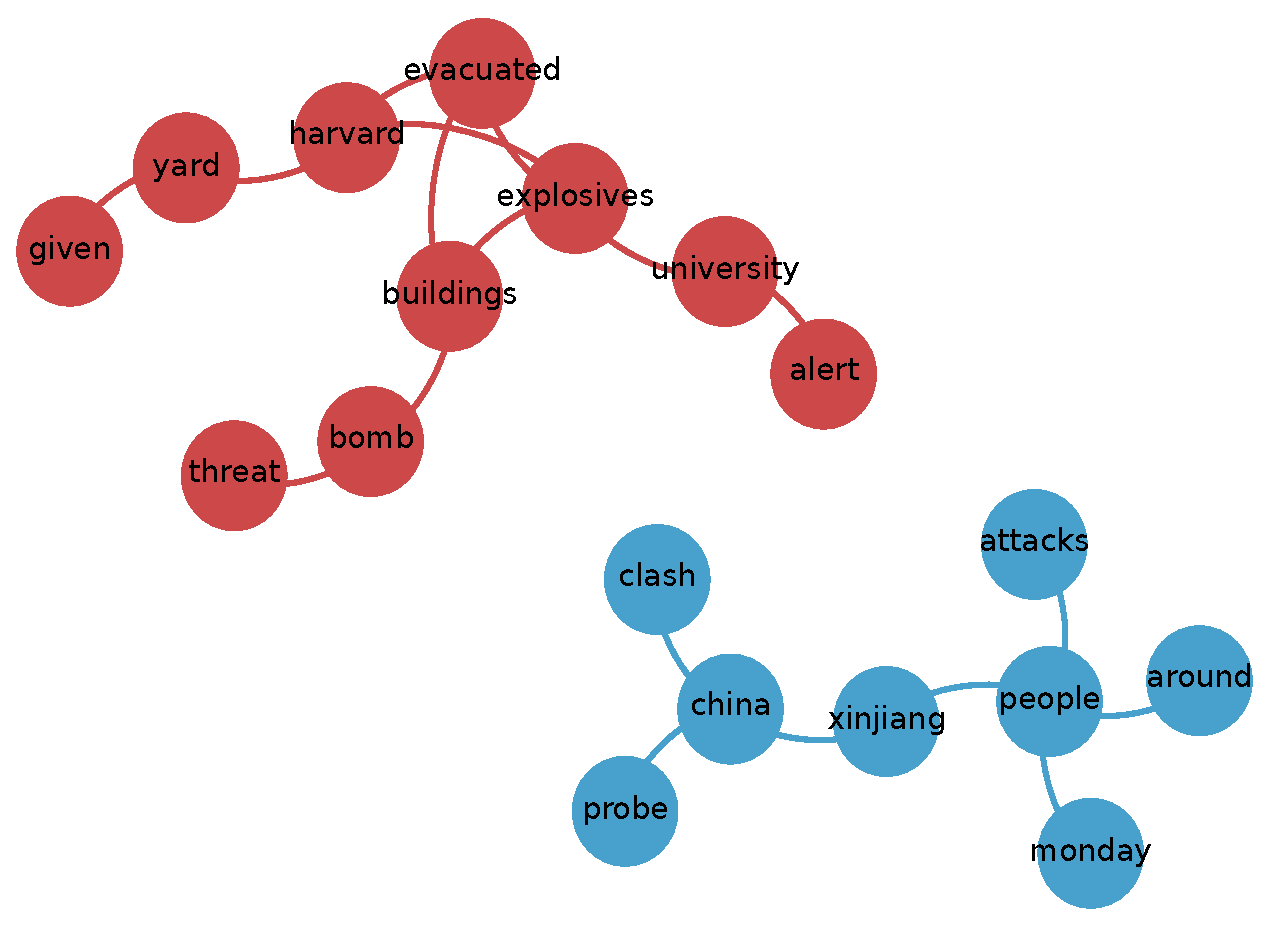
\includegraphics[width=.6\textwidth]{figures/data/connected_components.eps}
    \caption[Example of connected components]
    {Example of connected components. Two keyword sets are joined if they share
    at least one keyword in common.}\label{fig:connected-component}
\end{figure}



\section{Data Cleaning and Validation}\label{sec:cleaning}

There are two issues in our methodology: domain-specific stopwords and very old
tweets.

First, the event identification methodology does not take into account the use
of common words in the headlines. 
%
After removing the typical stopwords (words like ``the'', ``is'', ``do'', etc.),
some other common words appear in the headlines. 
%
Those words can be selected as the keywords for some news events, and by being
common, can join unrelated events together.
%
For example, words like ``update'' or ``breaking'' are commonly used by
different news sources. 
%
We validated our methodology by comparing the resulting events with random
events, those resulting from joining random keyword sets.

Second, due to the REST API behavior, some tweets are very old with respect to
the corresponding event. 
%
Sometimes the tweets are months or even years old. 
%
For that reason, we remove all tweets that were more than ten days old from the
date of the event. 

The event durations are then analyzed in order to verify if including the first
portion of the data, for each news event, makes sense in terms of their
duration. 
%
For instance, if the tweets are evenly distributed, the time span in the first
5\% of the total amount of tweets should be half the duration of the first 10\%,
one quarter of the 20\%, and so on. 
%
However, our data shows that, for example, the first few tweets of an event are
from two or more years previous to the occurrence, and the remaining tweets are
mainly concentrated closely around the date of the event.
%
The first 5\% of the tweets would then be significantly older than the rest
95\% in terms of time duration of the event. 


\subsection{Detecting Articulation Words}

A problem that arose during the data collection was that, sometimes unrelated
events were joined together with keywords that was common to both events.  
%
This happens when two or more headlines from different events share a common
keyword. 
%
We performed a simple approach to identify such words and remove them from the
process.

Typical stopwords were removed when detecting groups of keywords to perform
searches, but some other words were common among the news accounts queried. 
%
For example, words like ``watch'', ``live'', or ``update'' are common to express
things like ``watch this video'', ``we are live on TV'', or to update a previous
headline with more info about it. 
%
By being common to different events (for example: ``Watch Jim Harbaugh's press
conference
live''\footnote{\url{https://twitter.com/49ers/status/519202023628374016}
(Accessed: February 29, 2020)}  and ``WATCH LIVE: Of the 48 people being
monitored for contact with Dallas patient, no one is showing any
symptoms''\footnote{\url{https://twitter.com/PzFeed/status/519203692898435072}
(Accessed: February 29, 2020)}), they can end up in unrelated events by joining
the keywords by those stopwords.


One approach to dealing with this problem is to have a pre-defined list of
stopwords to remove from the stream of headlines. 
%
Although we do not know beforehand which words those are. 
%
We call such words \emph{articulation words} in the sense that if they appear as
keywords after processing a group of headlines, then when joining the searches
together, those words would join unrelated events. 

%%

Intuitively, if a word appears in all the documents, then its {\em
tf-idf}~\cite{sparck1972statistical} score is generally low in all the
documents.  
%
However, if the word appears in very few documents, its statistic in those
documents is fairly high, indicating that the word is somehow representative of
the content of the document. 
%
It turns out the articulation words do not occur often enough for them to be
detected by regular \emph{tf-idf}, but do occur enough times for them to falsely
relate several unrelated events together. 
%
To identify a group of those keywords, we used a modified \emph{tf-idf} to
detect them from the headlines.

The modified version of \emph{tf-idf}, what we refer to as \emph{maxtf-idf}, is
meant to assign more weight to the terms that are frequent in any document. 
%
For instance, \emph{tf-idf} of a term in a document tries to assign a weight
related to how ``rare'' that term is in the whole collection, and how frequent
it is in that document, by indicating how representative the term is with
respect to the document. 
%
On the other hand, what we want to achieve is to weigh a term more if it
is more frequent in any document, relative to the frequency in the current
document. 
%
With that in mind, we want to identify terms that might be ``adding noise'' to
the corpus, and hence, to join unrelated events together.

The definition of \emph{maxtf} is as follows:

\begin{equation}
\text{maxtf}(t,\mathit{d},D) = 0.5 + \frac{0.5 + max\{f(t,\mathit{d}') : \mathit{d}' \in D\}}{max\{f(w,\mathit{d}) : w \in \mathit{d}\}}
\end{equation}

and for \emph{idf}, the usual formula:

\begin{equation}
\text{idf}(t,D) = \log\frac{N}{|\{\mathit{d} \in D : t \in \mathit{d}\}|}
\end{equation}

\noindent where $t$ is a term, $\mathit{d}$ is a document, and $D$ is the corpus
of documents. 
%
In this case, we set $t$ as a keyword, $\mathit{d}$ as the set of keywords of
one hour, and $D$ the set of documents of that day.

\begin{figure}
\begin{center}
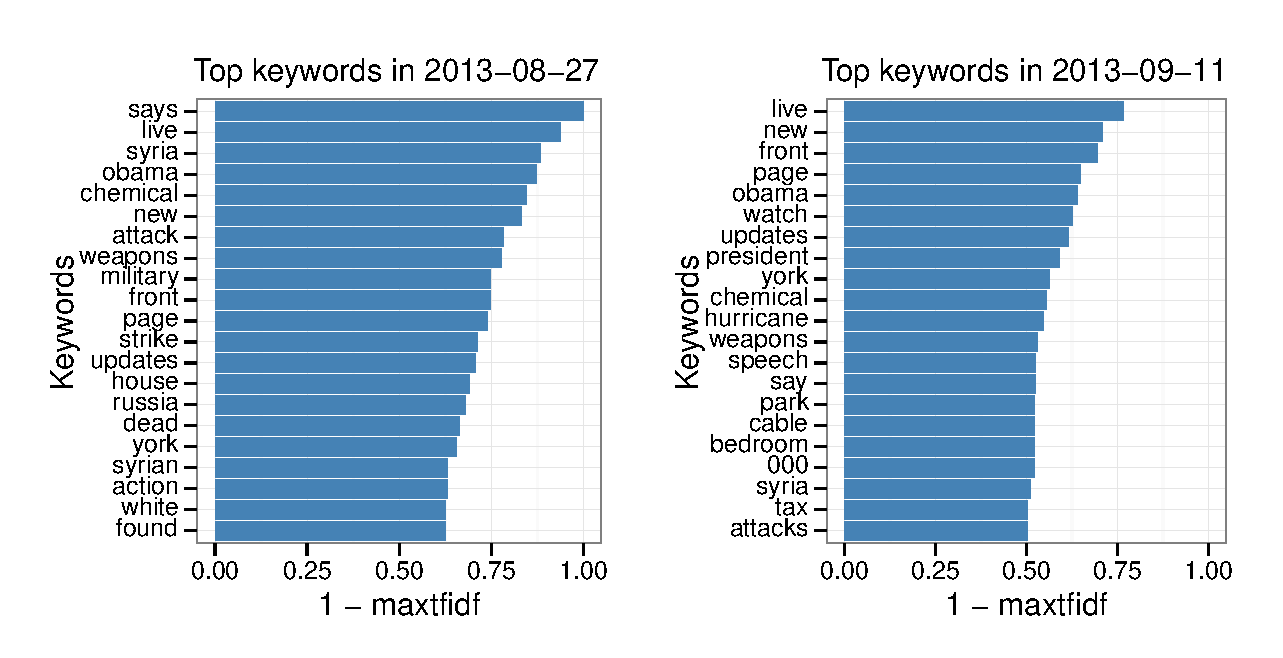
\includegraphics[width=\textwidth]{figures/data/stopwords}
\caption[Stopwords detection.]{Stopwords detection. Normalized
  $1-\text{maxtf-idf}$ score for data from August 27th (left) and August 28th
  (right) of 2013. The top score words for both plots are ``says'' and ``live''.
  We used the top score words to disconnect connected components of events. The
  title indicates the date when those keywords were identified, while the number
  beside corresponds to the total number of keywords.}
\label{fig:stopwords}
\end{center}
\end{figure}


After identifying such words, the idea was to disconnect the components
connected by those words. 
%
The process was to disconnect each component by the word with top normalized
$1-\text{maxtf-idf}$ score each time until the component could not be
disconnected further. 
%
We ended by adding the top score words to a list of banned words which were
ignored from subsequent runs of the data collection methodology. 
%
In Figure~\ref{fig:stopwords} there are two examples of this process to identify
the words.


\subsection{Validation of Event Modeling}\label{sub:valcoll}

In order to validate the results of the event identification process, we
compared our results with a baseline consisting on randomly generated events.

We generated artificially connected components taking randomly searches from the
first stage, and then merging their tweets to generate a ``random'' connected
component. 
%
The assumption here is that the tweets of a search are closely related to its
pair of keywords. 
%
From that, we wanted to ensure that the identified events make sense by
comparing them with random components. 
%
The idea is that using the connected components approach would join related
events together, so it would suffice to compare to a random baseline.

\begin{figure}
\begin{center}
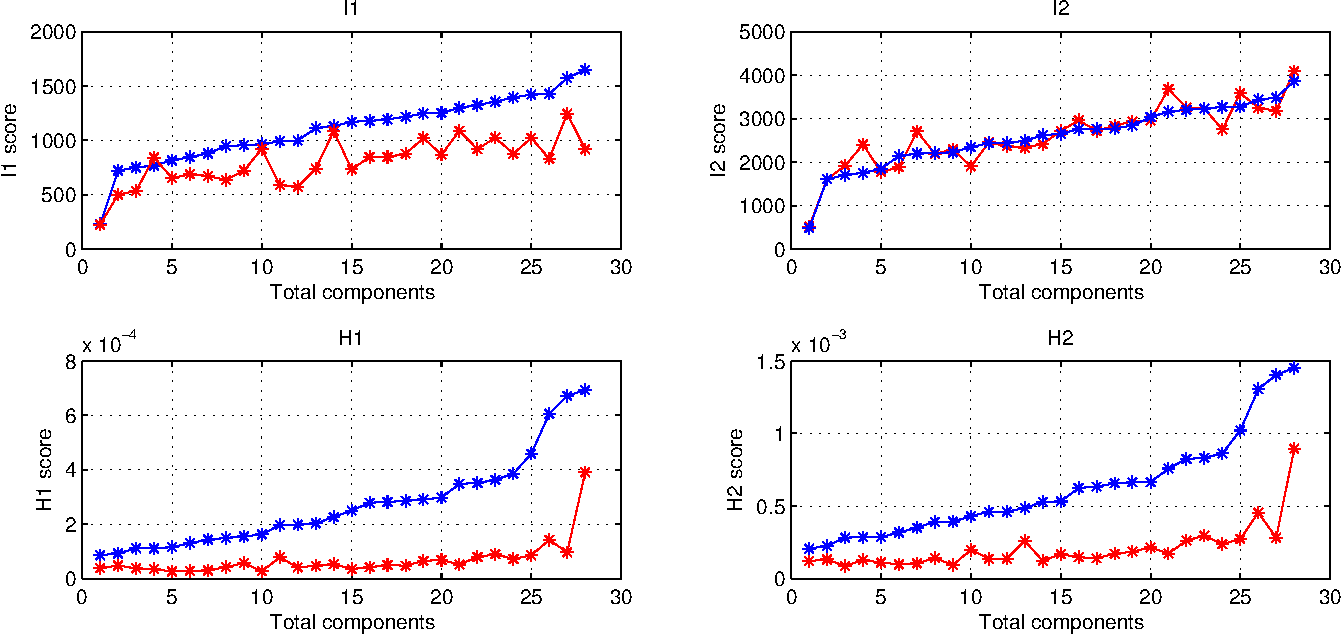
\includegraphics[width=.8\textwidth]{figures/data/connected_components_validation2.pdf}
\caption[Validation of connected components] {Validation of connected
  components. Each plot in this figure compares the quality of the cluster of
  tweets obtained from connected components and random components. The blue line
  corresponds to our approach, while the red line corresponds to the random
  components baseline. For visual clarity, the values obtained from connected
  components were sorted in ascending order, hence the blue line is
  monotonically increasing. The values obtained were rearranged in the same
  order as well.}\label{fig:connected_components_validation} 
\end{center}
\end{figure}

\begin{table}
\centering
\begin{tabular}{| c | c | c |}
\hline
Name & Metric & Meaning \\
\hline
\hline
$I_1$ & $\sum_{i=1}^k \frac{1}{n_i} \sum_{(u,v) \in S_i} \text{sim}(u,v)$ & Higher value is better\\
\hline
$I_2$ & $\sum_{i=1}^k \sqrt{ \sum_{(u,v) \in S_i} \text{sim}(u,v)}$ & Higher value is better \\
\hline
$E_1$ & $\sum_{i=1}^{k} n_i \frac{\sum_{v \in S_i, u \in S} \text{sim}(u,v)}{\sqrt{\sum_{(u,v) \in S_i} \text{sim}(u,v)}}$ & Lower value is better \\
\hline
$G_1$ & $\sum_{i=1}^k \frac{\sum_{v \in S_i, u \in S}\text{sim}(u,v)}{\sum_{(v,u) \in S}\text{sim}(v,u)}$ & Lower value is better \\
\hline
$G_1^{'}$ & $\sum_{i=1}^k n_i^2 \frac{\sum_{v \in S_i, u \in S}\text{sim}(v,u)}{\sum_{(u,v) \in S_i}\text{sim}(u,v)}$ & Lower value is better \\
\hline
$H_1$ & $\frac{I_1}{E_1}$ & Higher value is better \\
\hline
$H_2$ & $\frac{I_2}{E_1}$ & Higher value is better \\
\hline
\end{tabular}
\caption[Clustering metrics used for validation]{Clustering metrics used for
  validation. This table lists the clustering metrics used in Figure
  \ref{fig:connected_components_validation}. Those formulas correspond to usual
  clustering evaluation metrics, like inter-cluster similarity ($I_1, I_2$),
  intra-cluster similarity ($E_1, G_1, G_1'$) and similarity radio ($H_1, H_2$).
  In $I_1, I_2, H_1, H_2$ a higher value is better.  In $G_1, G_1^{'}$, lower
  value is better. }
\label{table:clustering_metrics}
\end{table}

We calculated standard internal clustering metrics~\cite{zhao2001criterion}
(listed in Table~\ref{table:clustering_metrics}) over the components and on the
random components and then compare their results. 
%
The comparisons were made by taking components of the same size (in terms of
keywords and tweets, taking samples of tweets). 
%
Essentially, considering a component as a cluster, the metrics evaluate the
similarity intra- and inter-clusters. 
%
We compare the metrics against random clusters to see if our approach tends to
join related events together, compared to a baseline.
%
Equal results mean that our approach is no better than joining searches
randomly. 
%
The results by metric are shown in
Figure~\ref{fig:connected_components_validation}. For almost every metric, our
approach is better than random.


\subsection{Event duration}\label{sub:dur}

Due to the capabilities of the REST API, the tweets collected can be older than
the actual date of the event detected. 
%
For that reason, some tweets can be very old and not relevant to the event
itself. 
%
Furthermore, when a retweet is collected by the process, also the original tweet
is stored\footnote{The data of the original tweet is included in the data of the
retweet}. 
%
This could be a problem especially when we want to perform predictions using the
first part of the data. 


\begin{figure}
\centering
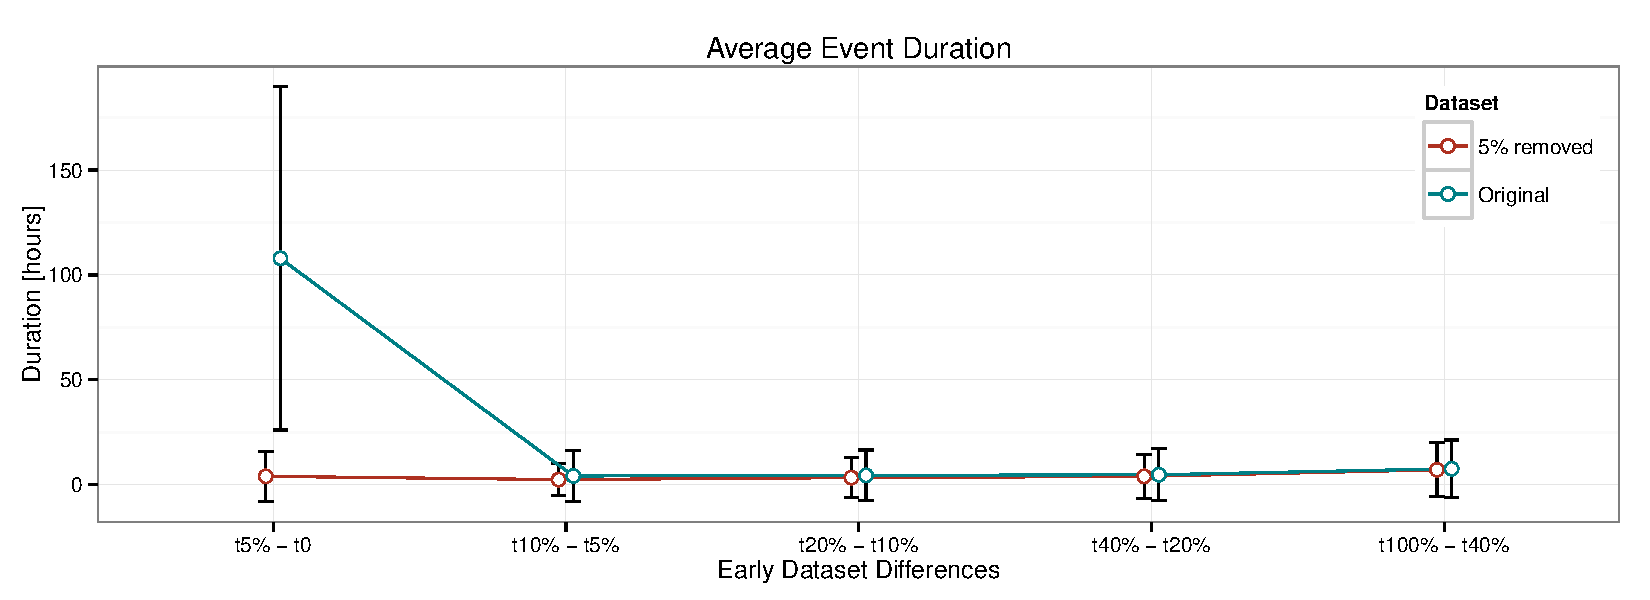
\includegraphics[width=\textwidth]{figures/data/duration-differences.pdf}
\caption[Duration differences of events.]{Duration differences of events. The
  $x$-axis represents the categories of datasets: the first one (t5\%-t0)
  represents the difference of time between the timestamp of the oldest tweet
  and the newest tweet on the first 5\% of the tweets. The next one (t10\%-t5\%)
  corresponds to the difference between the newest tweet in the first 10\% and
  the newest tweet on the first 5\% of data, etc. After removing the first 5\%
  of data, the time differences are roughly the same across all
  datasets.}\label{fig:duration-differences}

\end{figure}

After collecting tweets for an event, we remove the first 5\% of tweets of each
event, in addition to restrict tweets of an event up to ten days before the day
of its publication. 
%
We saw that the first 5\% of the tweets cover the largest amount of time on all
events, due to the problems exposed above. 
%
After removing the first 5\%, the events duration were more consistent (the
first 10\% covers twice the amount of time that the first 5\% covers, and so
on). 
%
Figure~\ref{fig:duration-differences} shows the effect of removing the first 5\%
of data by calculating the time differences between the timestamps of the tweets
at the ends of each dataset.


\begin{figure}[t]
  \centering
  \begin{subfigure}{\textwidth}
    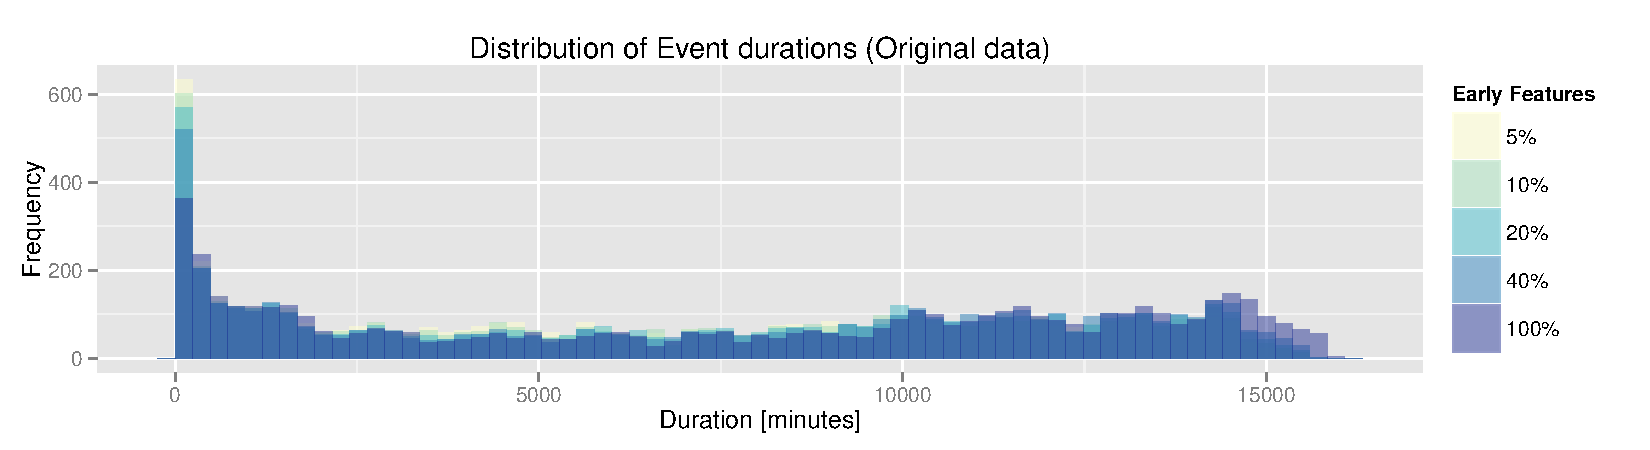
\includegraphics[width=\textwidth]{figures/data/dist-events-durations-o.pdf}
    \caption[Distribution of event duration on the original
      dataset.]{Distribution of event duration on the original dataset.} 
    \label{sfig:dist-events-durations-o}
  \end{subfigure}

  \begin{subfigure}{\textwidth}
    \centering
    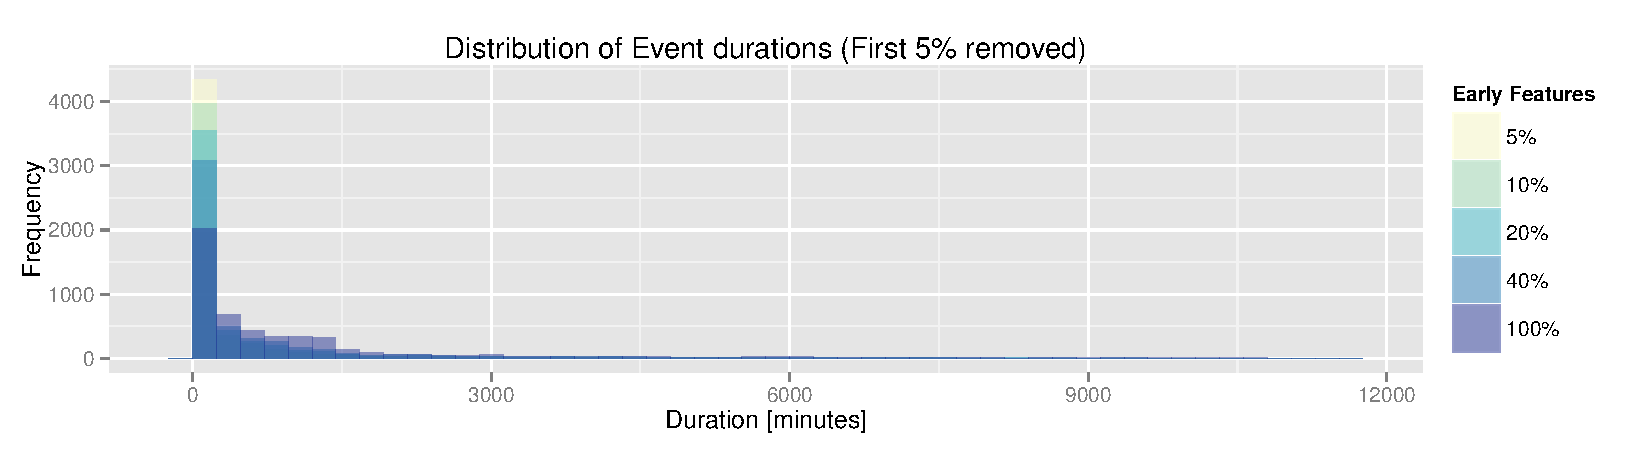
\includegraphics[width=\textwidth]{figures/data/dist-events-durations-5.pdf}
    \caption[Distribution of event duration on the 5\%-trimmed
      dataset.]{Distribution of event duration on the 5\%-trimmed dataset.} 
    \label{sfig:dist-events-durations-5}
  \end{subfigure}

  \caption[Distribution of event duration]{Distribution of event duration. In
    (a) we see that there is a non-negligible amount of events with a
    high duration (between 7 and 10 days). In (b), we see a clearer power law on
    the distribution of events after removing the first 5\% of tweets.}
  \label{fig:dist-events-durations}
\end{figure}

Event duration distributions are shown in
Figure~\ref{fig:dist-events-durations}. 
%
Figure~\ref{sfig:dist-events-durations-o} shows that there is a non-negligible
amount of events with a duration between 7 and 10 days. 
%
By considering the first 5\% of tweets from those events, the oldest tweets will
correspond to situations when the event has not already happened yet, and it
will lead to errors or incorrect results. 
%
Removing the first 5\% produces a cleaner dataset, as shown in
Figure~\ref{sfig:dist-events-durations-5}.


%%%
\paragraph{Summary.}
%
Our data collection methodology consisted of a pipeline starting at headline
retrieval from manually selected news sources, ending with event identification.

An event is a set of keywords with a set of tweets that talk about these
keywords.
%
The keywords can be seen as the event representatives. 
%
For example, the event \{chile, northern, iquique, tsunami, struck, warning,
earthquake, magnitude\} describes an earthquake that occurred in Chile on April
2th. 
%
However, a few challenges had to be addressed from this methodology.

Some keywords are common across several distinct events. 
%
For that reason, it was necessary to identify such words and remove them from
the keywords detection phase, for example, words like ``update'', ``watch'', or
``live'', which do not add any value to the meaning of any event. 

Finally, due to the nature of the methodology proposed, the tweet sets had to be
trimmed because of their long duration. 
%
Because of the Twitter REST API, sometimes tweets from long ago were retrieved,
but since they add only noise to our dataset, they were removed.

